\section{Realizarea experimentelor și analizarea acestora}

	Pentru a putea testa și analiza rezultatele obținute folosind modelul acustic propus de această lucrare am creat o modalitate interactivă pentru a putea vizualiza și compara rezultatele obținute de modelul nostru folosind platforma Unity pentru a gestiona și dezvolta un software de simulare acustică folosind un game engine. Am construit trei încăperi, două dreptunghiulare și una sferică, pornind de la forme de bază și materiale contrastante pentru a putea facilita vizualizarea rezultatelor. 
	
	În cadrul experimentelor realizate au fost folosite următoarele spații interioare 3D:
	
	\begin{itemize}
		\utb Cameră rectangulară cu dimensiunile: 4m lățime, 5m lungime și 3m înălțime - Camera 1 
		
		\utb Cameră rectangulară cu dimensiunile: 30m lățime, 30m lungime și 15m înălțime - Camera 2 
		
		\utb Cameră sferică cu raza egală cu 5m - Camera 3 
	\end{itemize}

	Această serie de experimente ia în considerare mai mulți parametrii esențiali în contextul modelului acustic, precum: numărul de raze ce va fi distribuit în încăpere, numărul maxim de reflexii pe care o rază le poate atinge, lungimea maximă pe care o poate avea o rază și pasul de frecvență.	
	
	În această lucrare vom considera următoarea serie de notații:
	\begin{itemize}
		\utb $S$ - sursă audio
		
		\utb $M$ - microfon 
	\end{itemize}

	Atunci când discutăm despre un punct în spațiu am considerat un sistem de coordonate în trei dimensiuni $(x,y,z)$, unde $x$ este axa ce reprezintă lungimea, $y$ este înălțimea, iar $z$ este lățimea.
	
	Pentru ca experimentele să fie relevante am considerat aceeași configurație și aceeași melodie ce va fi difuzată pentru toate încăperile. Configurația folosită va fi:
	
	\begin{itemize}
		\utb 100 000 de raze distribuite uniform pentru camerele dreptunghiulare și 10 000 în cazul încăperii sferice
		
		\utb maxim 10 reflexii pentru o rază
		
		\utb 200m distanța maximă pe care o rază o poate parcurge
		
		\utb 8192Hz numărul de pași de frecvență
	\end{itemize}

	Pentru rularea modelului acustic este nevoie să considerăm o serie de microfoane, întrucât dorim să analizăm sunetul în anumite poziții ale încăperilor. Astfel, în Camera 1 am considerat poziția sursei $S(0, 0, 0)$ și următoarele poziții pentru microfoane:
	
	\begin{itemize}
		\utb $M0(2, 1.6, 1.7)$, fiind la distanța de 3.07m de sursă
		
		\utb $M1(-1.5, 1.2, 1.7)$, fiind la distanța de 2.56m de sursă
		
	\end{itemize}

	În Camera 2, sursa $S$ se află la poziția $S(0, 2.5, 0)$ și am considerat următoarele valori pentru pozițiile microfoanelor: 
	
	\begin{itemize}
		\utb $M0(2, 1.6, 1.7)$, fiind la distanța de 3.07m de sursă
		
		\utb $M1(-1.5, 1.2, 1.7)$, fiind la distanța de 2.56m de sursă
		
		\utb $M2(1, 2, 13)$, fiind la distanța de 13.19m de sursă
	\end{itemize}

	Pentru Camera 3, sursa $S$ este poziționată în punctul $S(0, 0, 4)$. Am utilizat ecuația Cercului pentru a putea împrăștia uniform microfoanele în încăpere, obținând astfel următoarele valori pentru pozițiile microfoanelor:
	
	\begin{itemize}
		\utb $M0(4, 0, 0)$, fiind la distanța de 5.65m de sursă
		
		\utb $M1(2.8284, 0, 2.8284)$, fiind la distanța de 3.06m de sursă
		
		\utb $M2(-2.8284, 0, 2.8284)$, fiind la distanța de 3.06m de sursă
		
		\utb $M3(-4, 0, 4.8984)$, fiind la distanța de 4.09m de sursă
		
		\utb $M4(-2.8284, 0, -2.8284)$, fiind la distanța de 7.39m de sursă
		
		\utb $M5(-7.347, 0, -4)$, fiind la distanța de 10.86m de sursă
		
		\utb $M6(2.8284, 0, -2.8284)$, fiind la distanța de 7.39m de sursă
	\end{itemize}


	Mediul în care trăim conține suprafețe și materiale, care absorb sau reflectă sunetul, fapt care atenuează sau împrăștie ceea ce noi auzim. Posibilitatea de a întâłni suprafețe care să absoarbă sau să reflecte total sunetul este una foarte mică, de obicei, acest lucru se întâmplă doar în condiții de laborator. 
	
	În funcție de suprafețe, coeficientul de absorbție diferă foarte mult, de obicei, obiecte precum covoarele, pânzele, pernele, absorb sunetul mult mai bine decât materiale precum lemnul, betonul, poliesterul. Astfel, am dorit ca soluția modelului acustic să fie una cât mai realistă și am considerat pentru toate suprafețele din încăperi o serie de coeficienți de absorbție. În cadrul experimentelor realizate, am ales coeficientul de absorbție 0.2.

	În Figura \ref{fig:Fig20} putem vizualiza cele trei încăperi, microfoanele și sursa audio realizate cu ajutorul platformei Unity. Se poate observa că prima încăpere este mai mică decât cea de-a doua și că cele două spații sunt similare. Pentru Camera 3, se consideră distribuirea uniformă a microfoanelor folosind ecuația cercului.
	
	\begin{figure}[!htb]%
		\begin{subfigure}[b]{.3\textwidth}
			\centering
			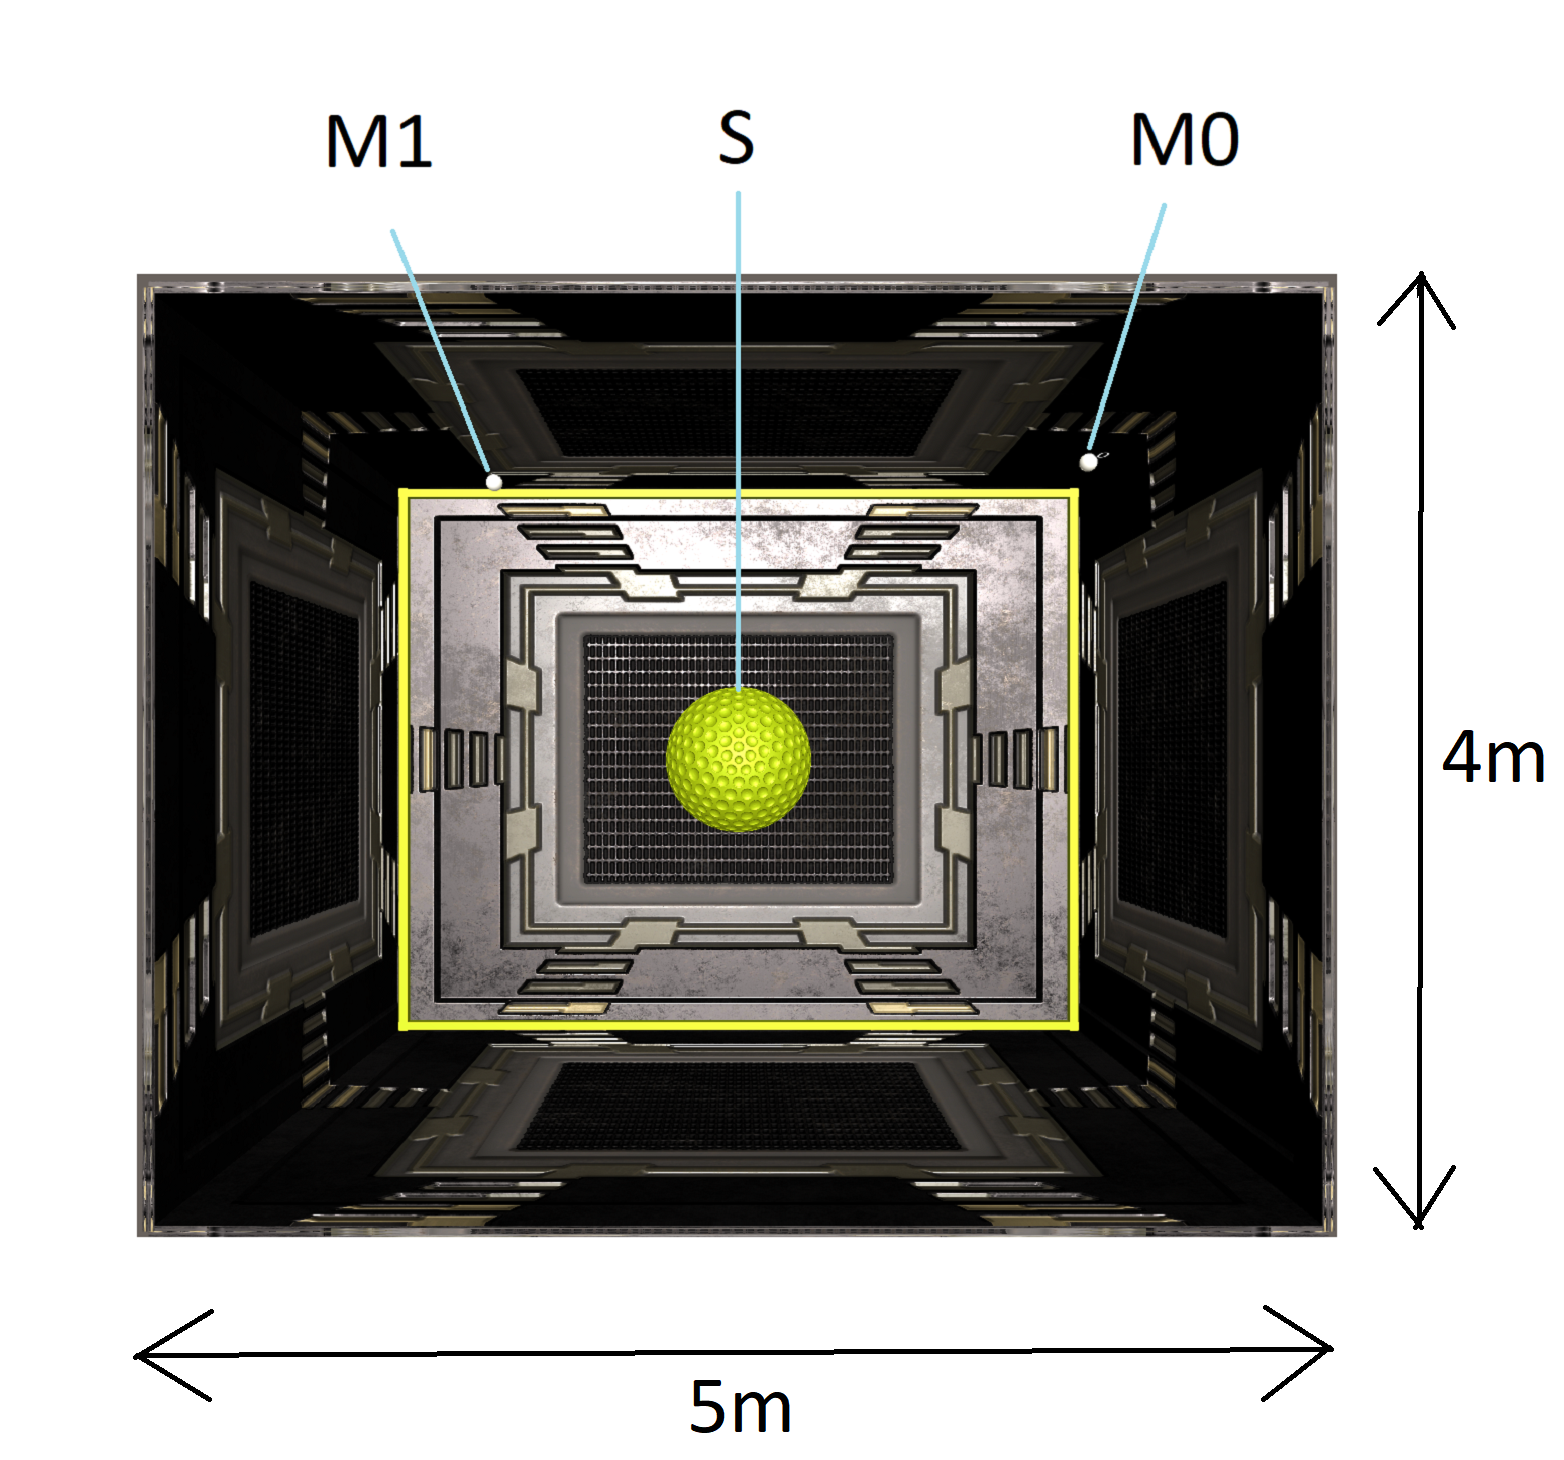
\includegraphics[width=1\linewidth]{imagini/roomA.png} 
			\caption{Camera 1}
			\label{fig:sub-fig}
		\end{subfigure}
		\hfill
		\begin{subfigure}[b]{.3\textwidth}
			\centering
			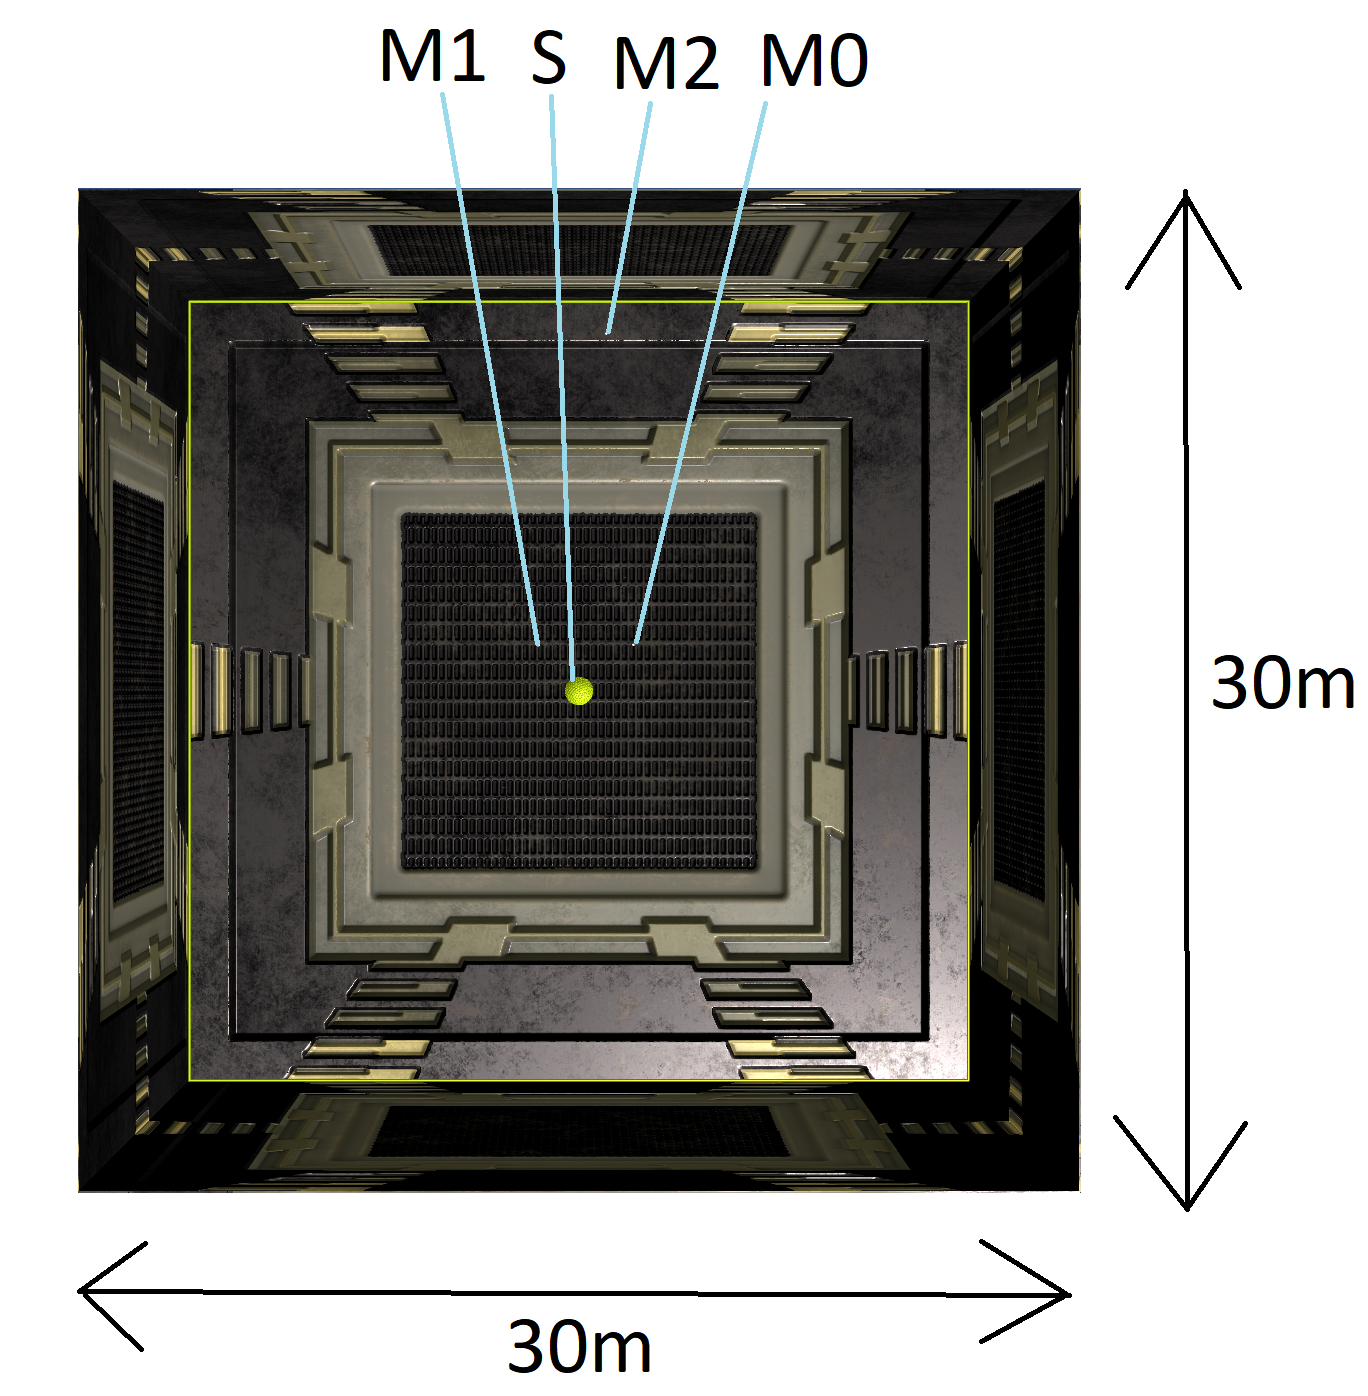
\includegraphics[width=1\linewidth]{imagini/roomB.png}
			\caption{Camera 2}
			\label{fig:sub-second}
		\end{subfigure}
		\hfill
		\begin{subfigure}[b]{.3\textwidth}
			\centering
			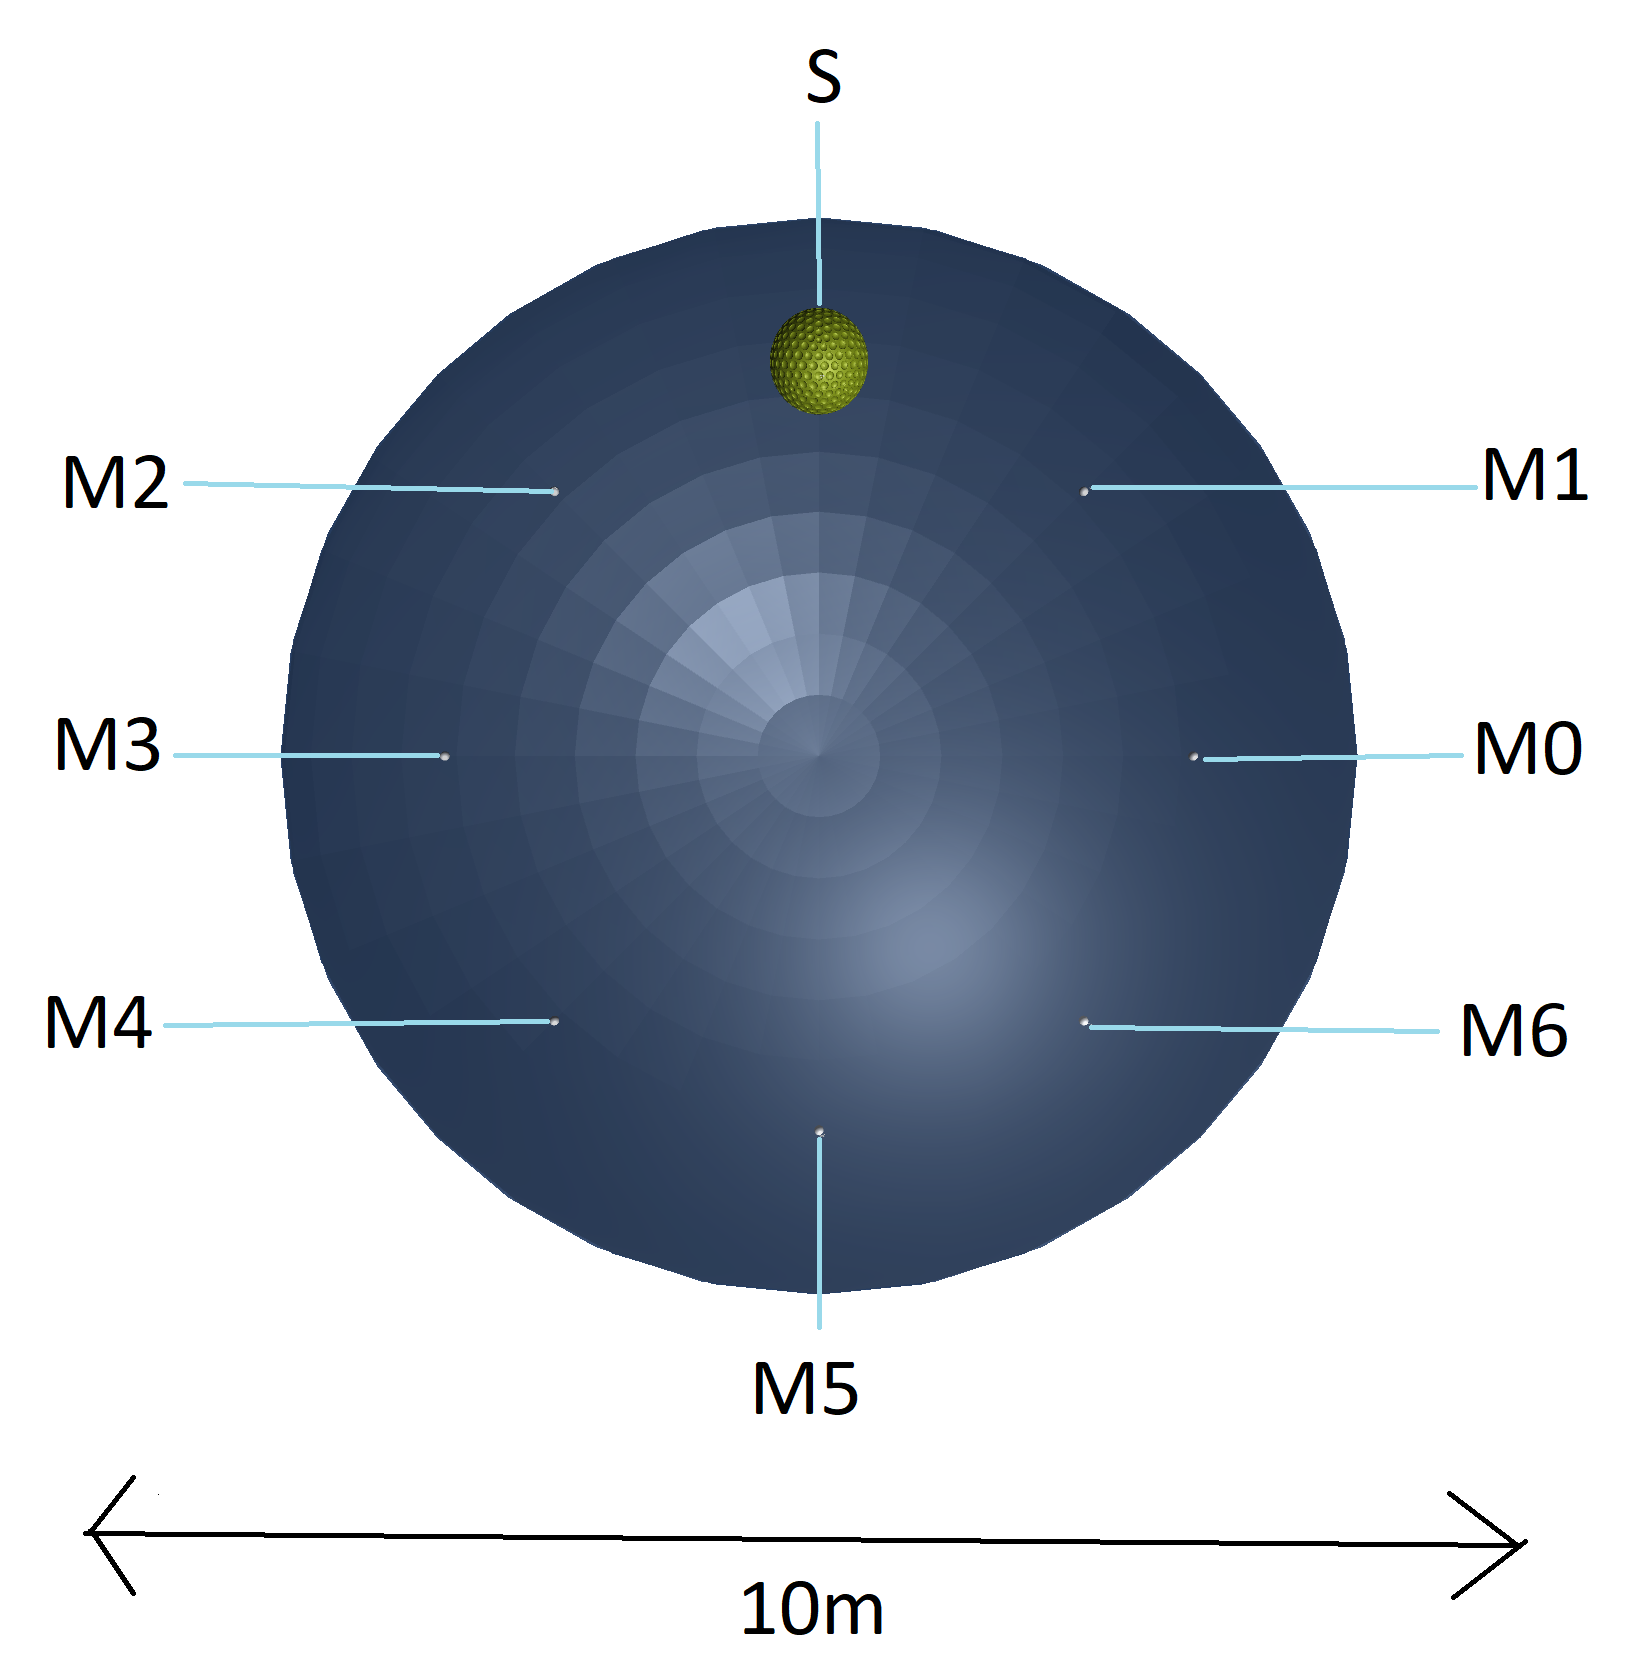
\includegraphics[width=1\linewidth]{imagini/roomC.png}
			\caption{Camera 3}
			\label{fig:sub-third3}
		\end{subfigure}
		
		\caption{Încăperile folosite pentru a realiza experimentele}
		\label{fig:Fig20}
	\end{figure}
	
	Putem observa în cazul Subfigurii \ref{fig:sub-fig} că datorită configurației potrivite este acoperită cea mai mare parte din suprafața încăperii, nefiind prezente ,,spații goale'', semn care indică faptul că sunetul a fost împrăștiat în toată camera și că poate fi auzit peste tot.
	
	Subigura \ref{fig:sub-second} ilustrează cea de-a doua încăpere și razele ce au fost distribuite în aceasta. Datorită configurației alese și a pozițiilor microfoanelor putem observa că multe porțiuni ale camerei au rămas neparcurse.
	
	În Subfigura \ref{fig:sub-third3} putem observa că datorită configurației potrivite și al modului simetric în care au fost plasate microfoanele razele au fost împrăștiate în încăpere în mod uniform.
	
	Figura \ref{fig:Fig21} prezintă unul din modurile de vizualizare al razelor din aplicație. În aceste imagini a fost utilizată configurația parametrilor, poziționarea microfoanelor și a sursei audio prezentate mai sus. 

	\begin{figure}[!htb]%
		\begin{subfigure}[b]{.3\textwidth}
			\centering
			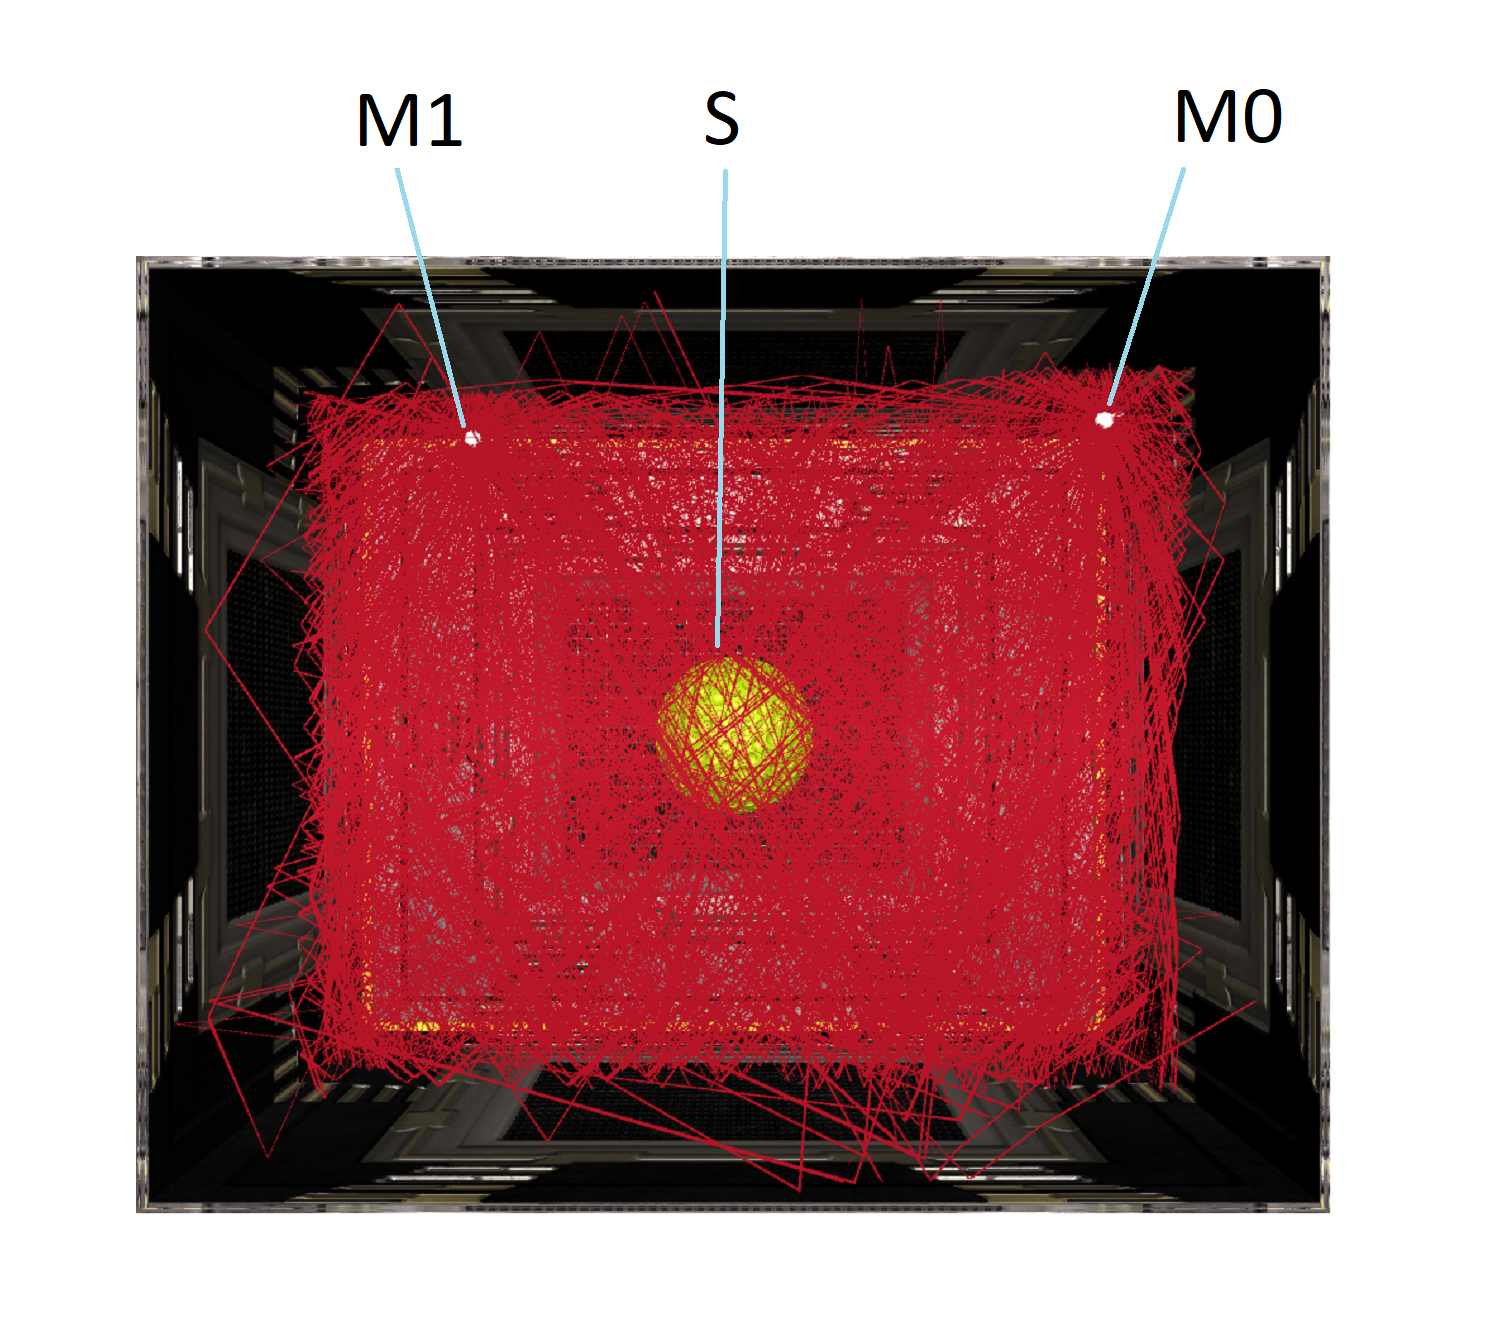
\includegraphics[width=1\linewidth]{imagini/roomA_rays.png} 
			\caption{Camera 1}
			%\label{fig:sub-fig}
		\end{subfigure}
		\hfill
		\begin{subfigure}[b]{.3\textwidth}
			\centering
			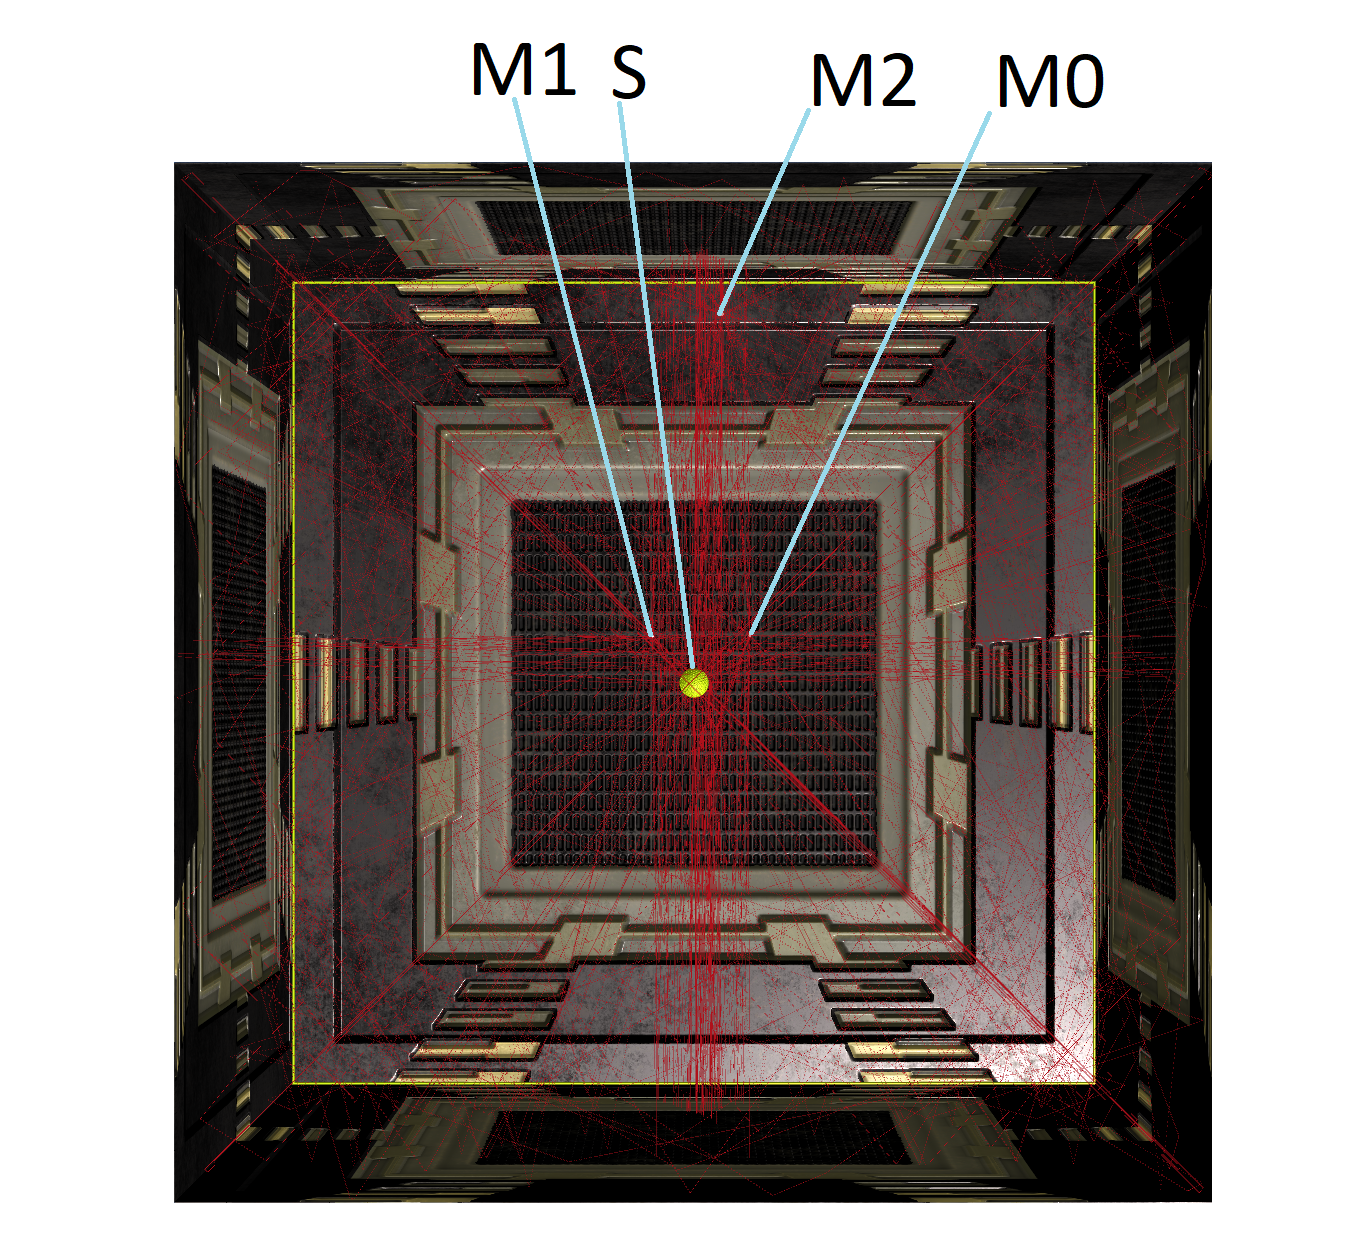
\includegraphics[width=1\linewidth]{imagini/roomB_rays.png}
			\caption{Camera 2}
			%\label{fig:sub-second}
		\end{subfigure}
		\hfill
		\begin{subfigure}[b]{.3\textwidth}
			\centering
			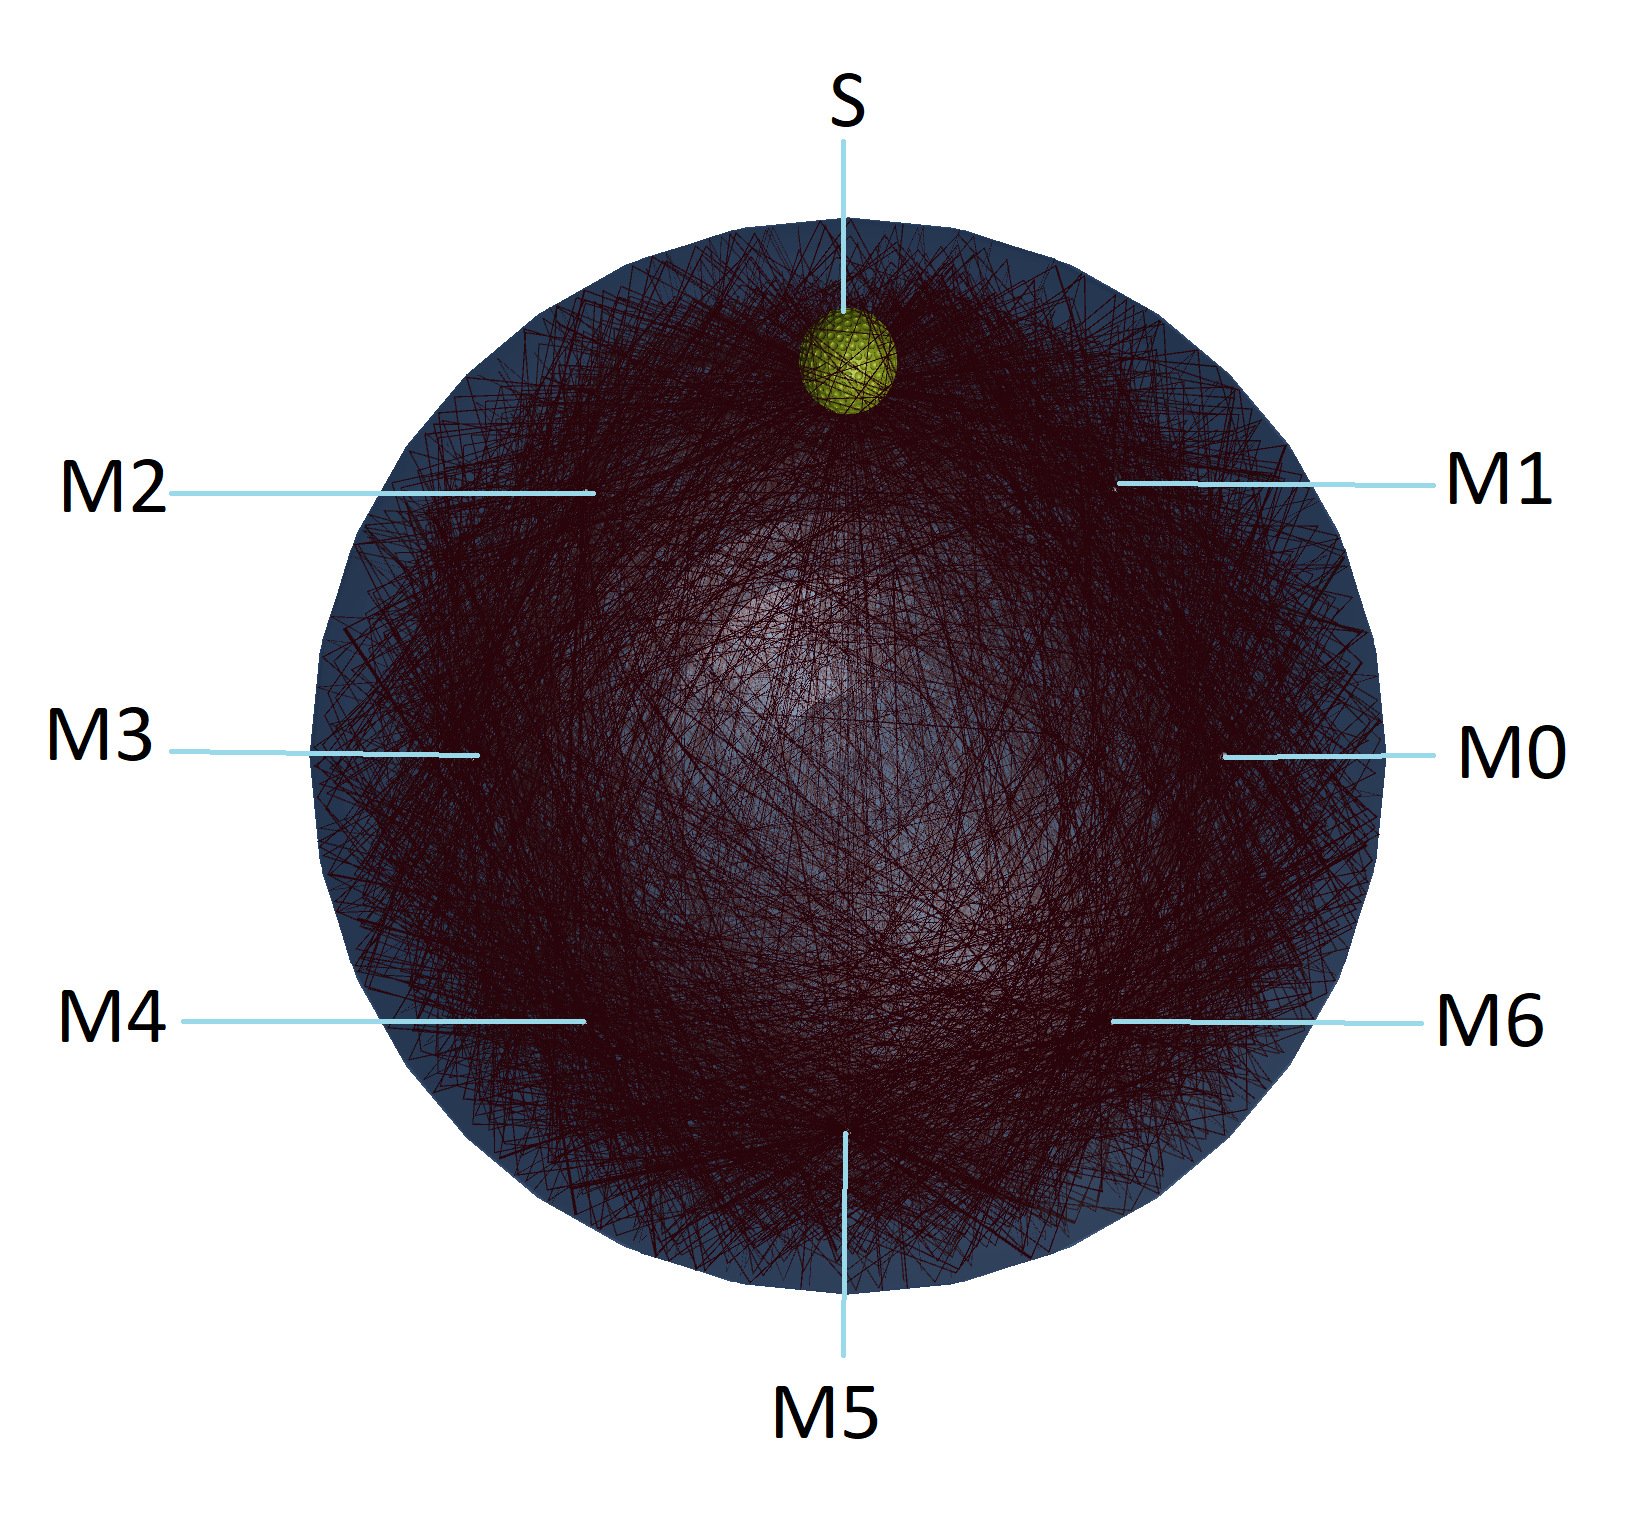
\includegraphics[width=1\linewidth]{imagini/roomC_rays.png}
			\caption{Camera 3}
			\label{fig:sub-third}
		\end{subfigure}
		
		\caption{Vizualizarea tuturor razelor din fiecare încăpere}
		\label{fig:Fig21}
	\end{figure}

	De asemenea, am realizat și un experiment în Camera 3 care presupune plasarea unui obstacol sferic între microfoanele $M4$ și $M5$ pentru a putea vedea dacă în acest mod sunt afectate rezultatele folosind modelul acustic. Pentru model am considerat aceeași configurație ca cea pentru Camera 1 și Camera 2, cu diferența că în încăperea sferică am considerat numărul de raze egal cu 10 000. În urma calculelor efectuate, am descoperit că 442 de raze au ajuns, în total, pe microfoane în cazul expus de Subfigura \ref{fig:sub-third} și
	378 în cazul expus de Subfigura \ref{fig:sub-third2}. Mai mult, am observat că, în cazul în care avem un obstacol în cameră, razele sunt
	mai împrăștiate și că anumite porțiuni nu sunt atât de dense, deoarece datorită obstacolului sunt create noi căi de propagare.
	
	Pe baza situațiilor prezentate mai sus putem vedea că în cazul încăperilor dreptunghiulare pe colțurile camerelor razele ajung mai greu, în timp ce în cazul încăperilor sferice razele ajung mai greu la centrul sferei.
	
	Dacă numărul de raze va fi prea mic în comparație cu dimensiunea camerei noastre, nu vom putea propaga sunetul foarte bine, deoarece există posibilitatea ca foarte puține raze sau chiar nici una să ajungă pe unul dintre microfoanele plasate în cameră. Deci, cu cât dimensiunea camerei este mai mare, cu atât este mai mare numărul de raze care vor fi distribuite în cameră și același lucru se întâmplă pentru numărul de reflexii și pentru lungimea maximă posibilă a unei raze.
	
	\begin{figure}[!htb]%
		\begin{subfigure}[b]{.3\textwidth}
			\centering
			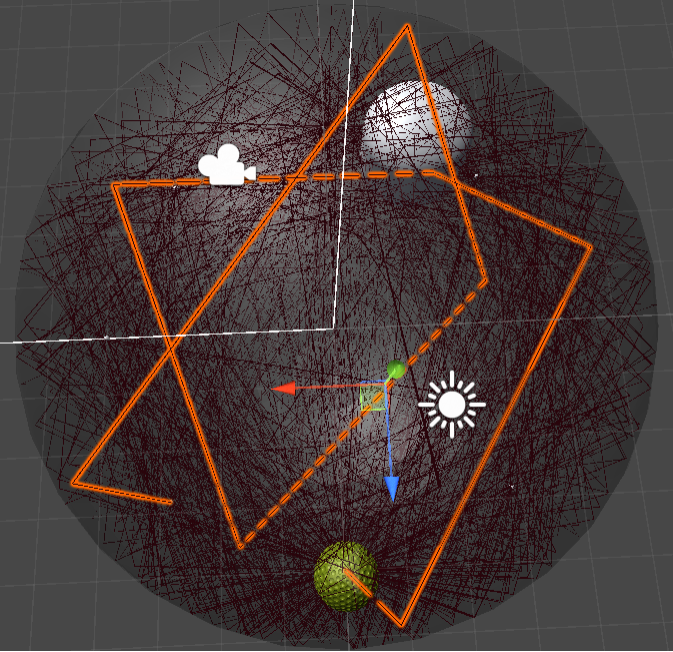
\includegraphics[width=1\linewidth]{imagini/m1r22-5000.png} 
			\caption{Raza trece pe deasupra, dar și lovește obstacolul}
			%\label{fig:sub-fig}
		\end{subfigure}
		\hfill
		\begin{subfigure}[b]{.3\textwidth}
			\centering
			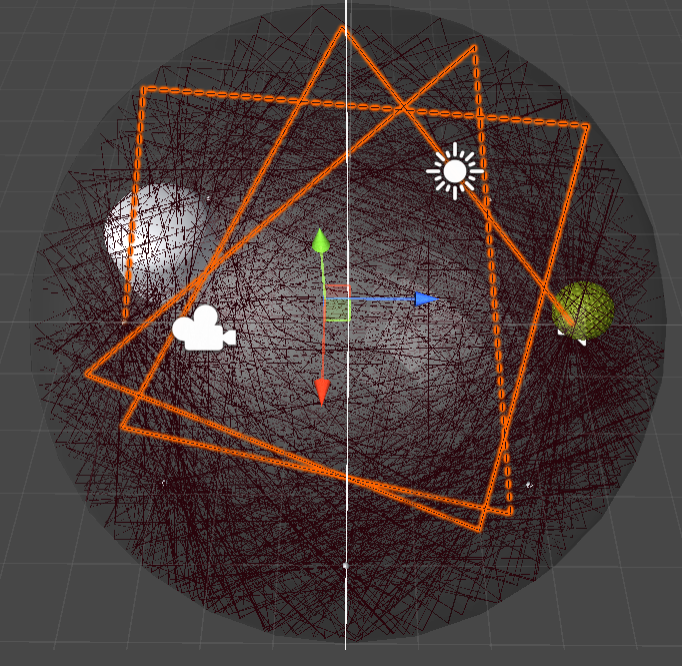
\includegraphics[width=1\linewidth]{imagini/m6r135-5000.png}
			\caption{Raza nu lovește deloc obstacolul}
			%\label{fig:sub-second}
		\end{subfigure}
		\hfill
		\begin{subfigure}[b]{.3\textwidth}
			\centering
			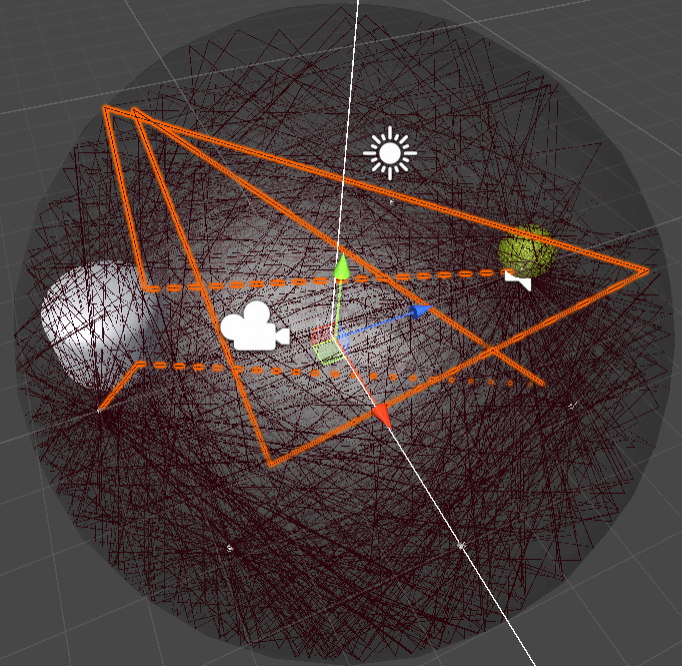
\includegraphics[width=1\linewidth]{imagini/m6r124-5000.png}
			\caption{Raza lovește de mai multe ori obstacolul}
			\label{fig:sub-third2}
		\end{subfigure}
		
		\caption{Diferite scenarii ale razelor}
		\label{fig:Fig22}
		
	\end{figure}

	Urmărind Figura \ref{fig:Fig22} putem observa că atunci când plasăm un obstacol în încăpere putem să ne aflăm în una dintre următoarele situații atunci când discutăm despre calea pe care o rază o parcurge: raza poate lovi sau nu obstacolul, poate trece pe deasupra sau pe dedesubtul acestuia.
	
	\begin{figure}[!htb]
		\centering
		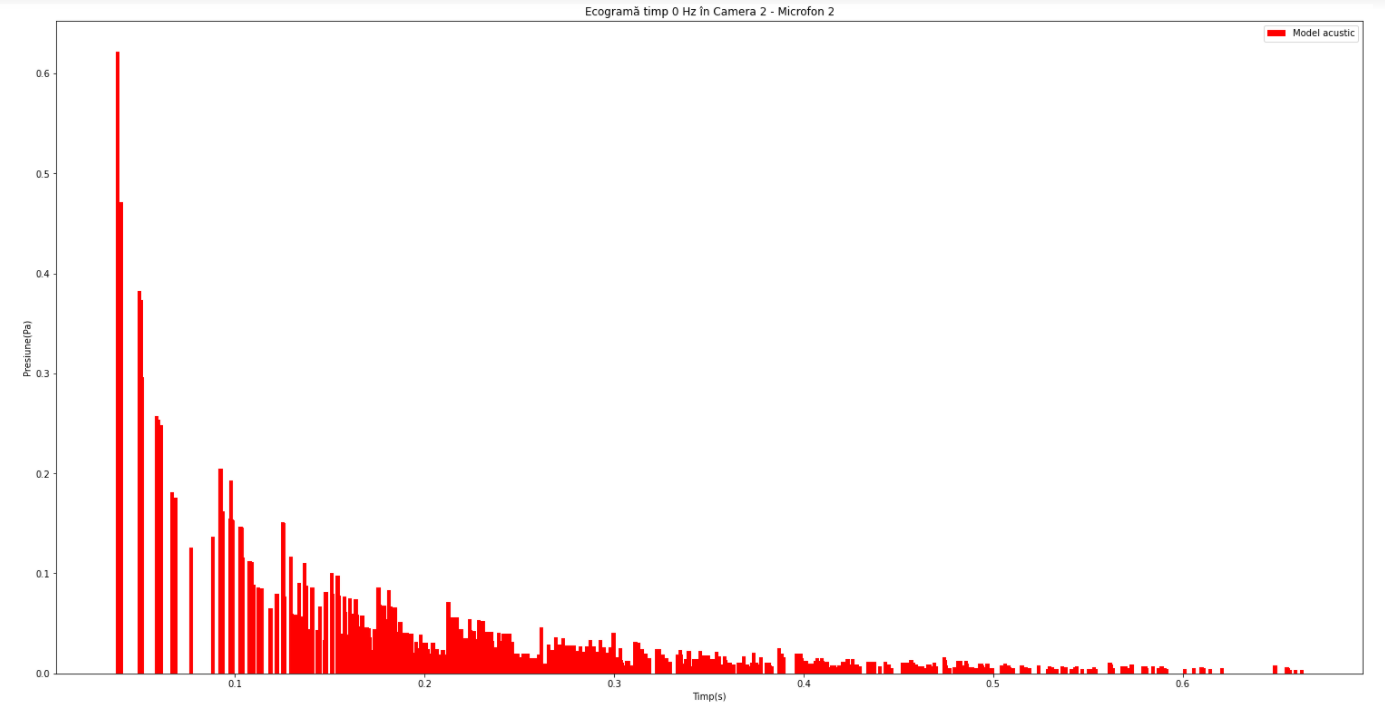
\includegraphics[width=1\linewidth]{imagini/ecograma.png}
		\caption{Ecogramă timp pe microfonul $M2$ în Camera 2}
		\label{Fig23}
	\end{figure}
	
	Considerând aceste cazuri de propagare al razelor în încăperea sferică putem trage concluzia că razele pot avea căi foarte diferite de a ajunge la microfon și că atunci când distanța unei raze de la sursa audio la microfon este foarte mare și sunetul va ajunge mai târziu.
	
	Atunci când discutăm despre ecograma în timp a unui microfon ne vom referi la graficul ce descrie presiunea și timpul. Se poate observa că Figura \ref{Fig23} conține o serie de bare verticale, unde fiecare bară reprezintă una dintre razele ce au ajuns pe microfonul 2 în Camera 2. Prima bară se caracterizează printr-o presiune crescută, deoarece corespunde razei care ajunge de pe sursă pe microfon în mod direct, fără a mai lovi alte suprafețe din încăpere. După această rază, urmează toate celelalte raze care au ajuns pe microfonul 2. Ordinea va fi dată de către numărul de reflexii și de către momentul în care raza ajunge pe microfon. Astfel, vom avea mai întâi raza directă, iar mai apoi razele care au o reflexie, după aceea două și așa mai departe până ajungem la raze ce au 10 reflexii.

	\begin{figure}[!htb]%
		\begin{subfigure}[b]{0.95\textwidth}
			\centering
			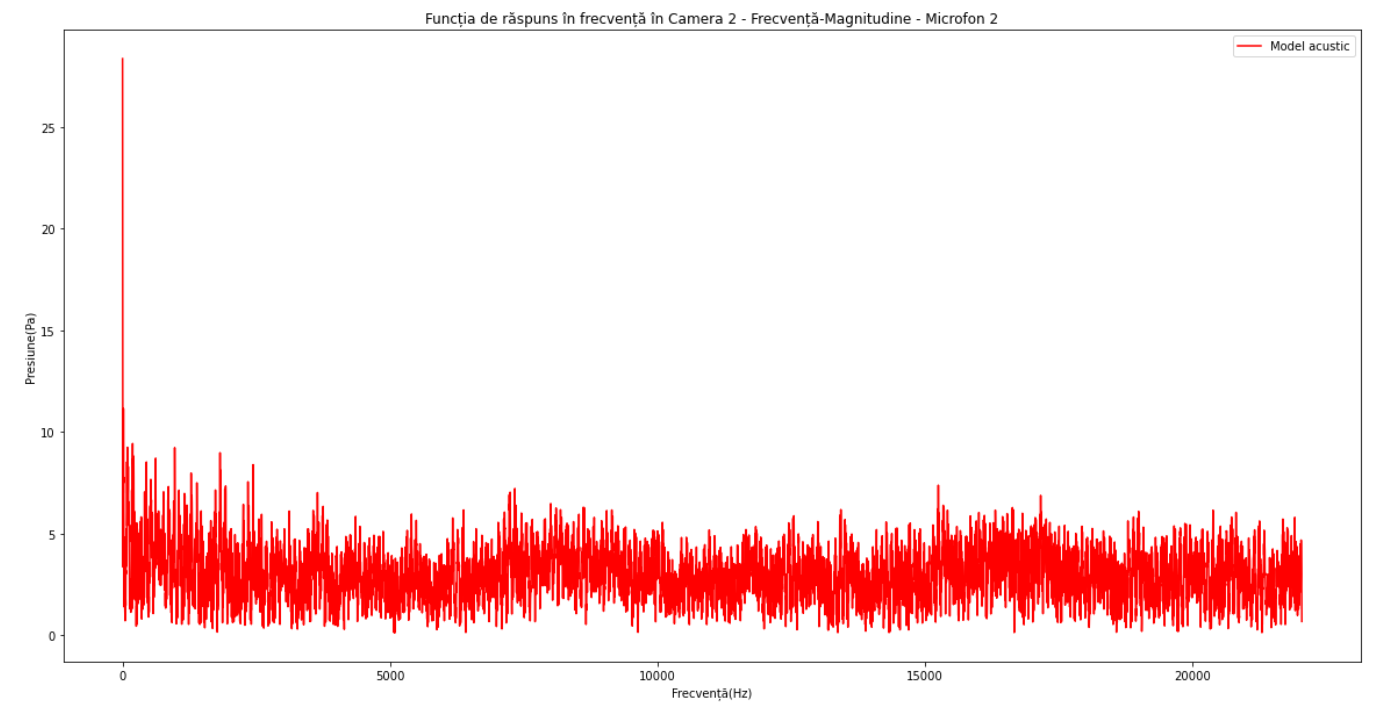
\includegraphics[width=1\linewidth]{imagini/fr_mag.png} 
			\caption{Grafic Frecvență-Magnitudine pe microfonul $M2$ în Camera 2}
			%\label{fig:sub-fig}
		\end{subfigure}
		\vfill
		\begin{subfigure}[b]{0.95\textwidth}
			\centering
			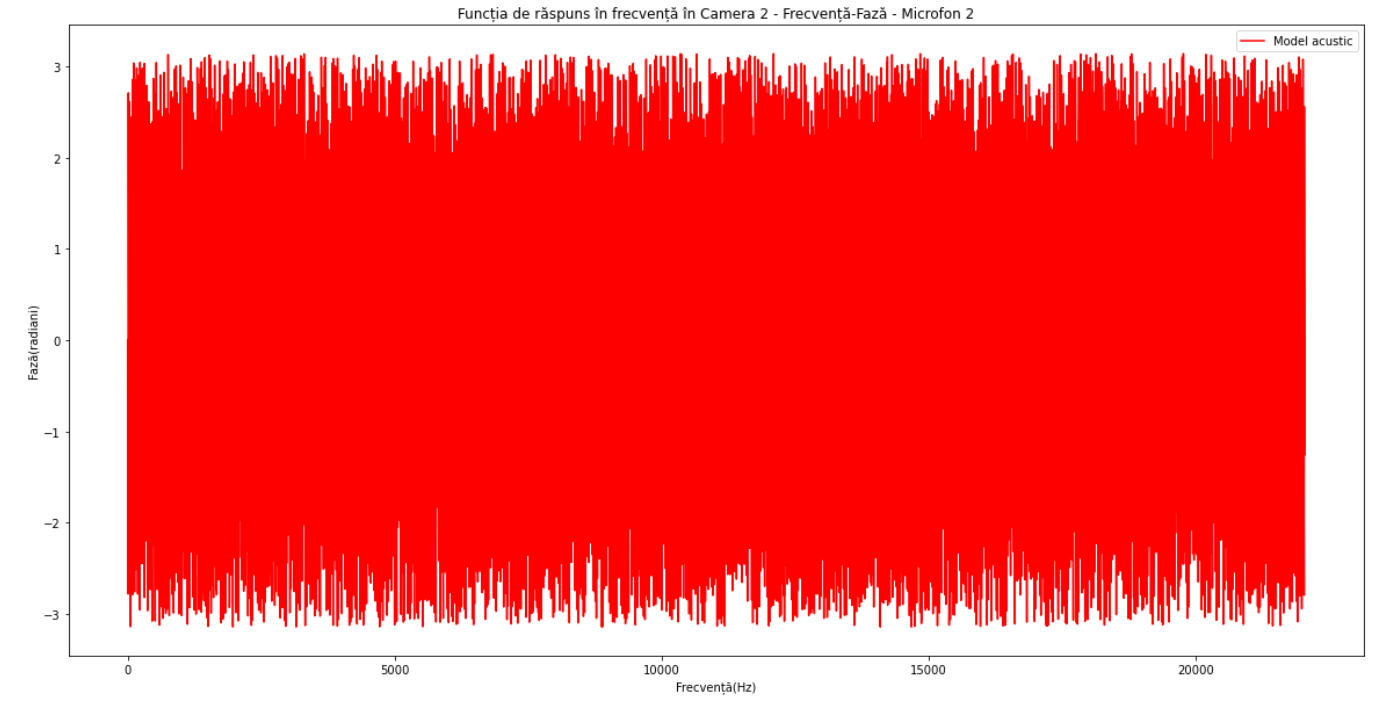
\includegraphics[width=1\linewidth]{imagini/fr_faza.png}
			\caption{Grafic Frecvență-Fază pe microfonul $M2$ în Camera 2}
			%\label{fig:sub-second}
		\end{subfigure}
		
		\caption{Funcția de răspuns în frecvență pe microfonul $M2$ în Camera 2}
		\label{fig:Fig24}	
	\end{figure}

	Funcția de răspuns în frecvență este măsura cantitativă a spectrului de ieșire al unui sistem sau dispozitiv ca răspuns la un stimul și este utilizat pentru a caracteriza dinamica sistemului. În termeni simpli, dacă o undă sinusoidală este injectată într-un sistem la o frecvență dată, un sistem liniar va răspunde la aceeași frecvență cu o anumită magnitudine și un anumit unghi de fază relativ la intrare.
	
	Funcția de răspuns în frecvență are, în general, valori complexe, cu părți reale și imaginare. Acest lucru este adesea mai util și mai intuitiv atunci când este exprimat în coordonate polare. Adică îl putem separa în magnitudinea sa (numită răspuns de amplitudine) și în
	componentă de fază (numită răspuns de fază).
	
	Reprezentarea domeniului de frecvență al unui semnal conține informații despre magnitudinea și faza semnalului la fiecare frecvență. Acesta este motivul pentru care ieșirea calculului FFT (Fast Fourier Transform) este complexă. Ieșirea FFT este un vector complex care conține informații despre conținutul de frecvență al semnalului. Faza prezintă modul în care se aliniază componentele de frecvență în timp. Aceste lucruri pot fi vizualizate în Figura \ref{fig:Fig24}, în cazul microfonului 2 din Camera 2.

	În procesarea semnalului, un răspuns la impuls este ieșirea unui sistem atunci când alimentăm sistemul cu un impuls ca semnal de intrare. Un impuls este orice semnal de scurtă durată. Cu toate acestea, în procesarea semnalului folosim, de obicei, o funcție Dirac Delta pentru sistemele analogice/continue. Pentru microfonul 2 din Camera 2 am obținut funcția de răspuns la impuls prezentată în Figura \ref{ir}, unde putem observa suișuri și coborâșuri ce ilsutrează fenomenul de ecou. 
	
	\begin{figure}[!htb]
		\centering
		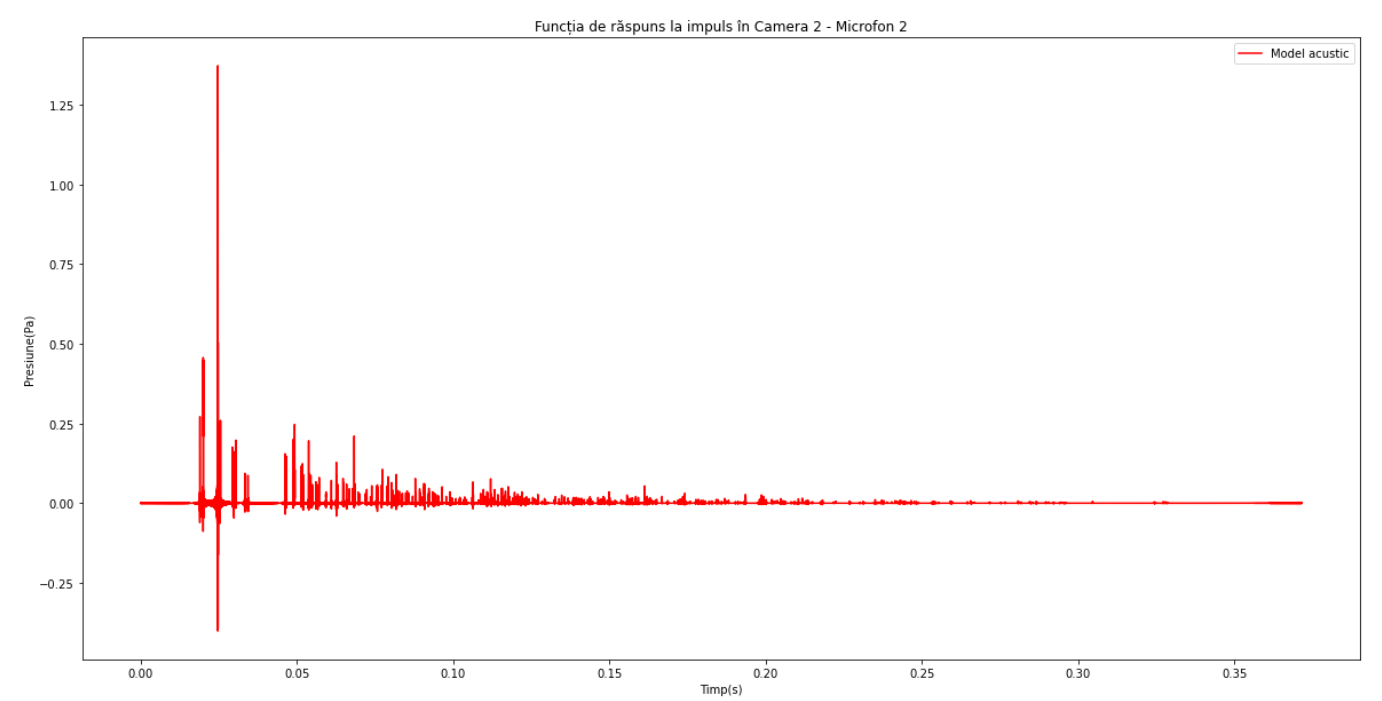
\includegraphics[width=1\linewidth]{imagini/ir.png}
		\caption{Funcția de rășpuns la impuls pe $M2$ în Camera 2}
		\label{ir}
	\end{figure}
	
	Pentru a putea analiza care este diferența de timp cu care ajunge semnalul pe microfoane am realizat un experiement care presupune desenarea tuturor punctelor obținute după pasul de convoluție. În Figura \ref{Fig25} putem observa semnalele rezultate pe toate microfoanele din Camera 2, unde semnalul ajunge cel mai repede pe microfonul 1, fiind la o distanță de 2.56m de sursă, apoi la o distanță foarte mică de timp pe microfonul 0, aflat la 3.07m de sursă, iar în cele din urmă ajunge pe microfonul 2, care este plasat la o distanță de 13.19m de sursă. Concluzionând, cu cât microfonul se află mai departe de sursa audio, cu atât razele vor parcurge un drum mai lung în încăpere și sunetul va ajunge mai târziu pe microfon.
		
	\begin{figure}[!htb]
		\centering
		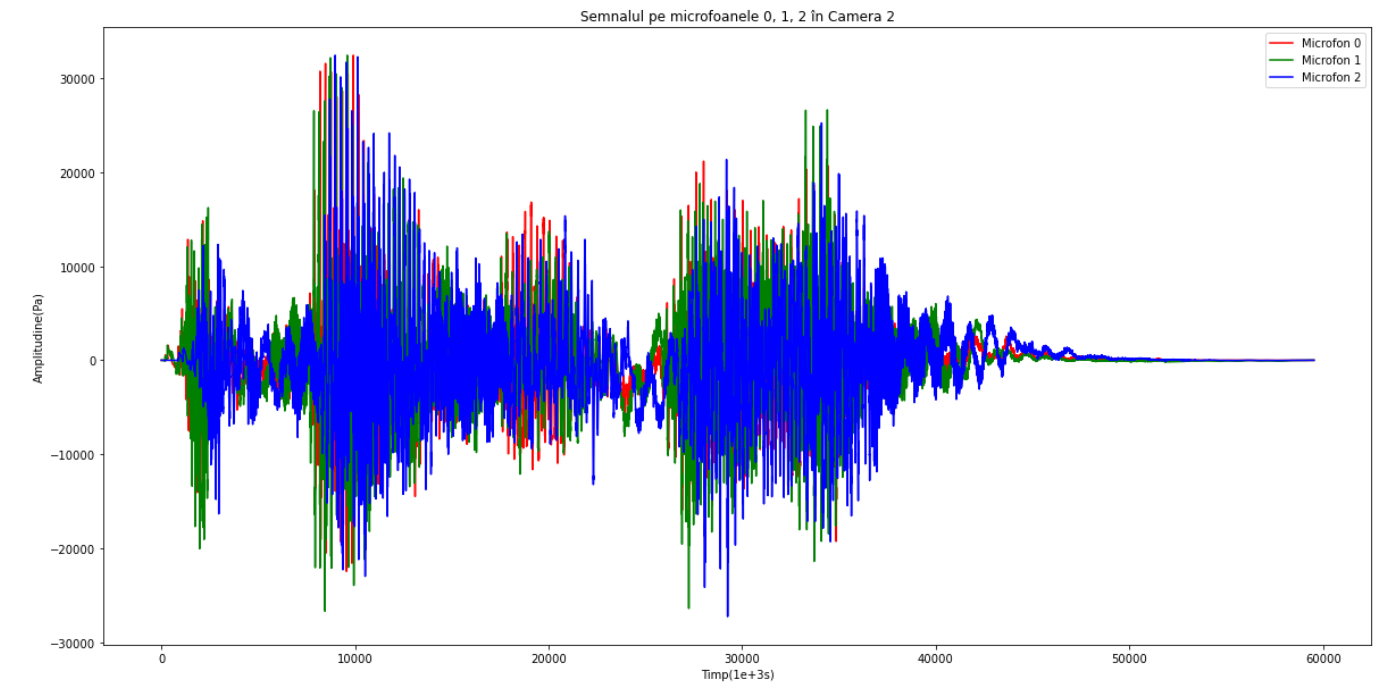
\includegraphics[width=1\linewidth]{imagini/sound.png}
		\caption{Semnalele rezultate pe microfoanele $M0, M1, M2$ în Camera 2}
		\label{Fig25}
	\end{figure}
		
	În contextul unei aplicații în care sunt implicate foarte multe calcule o etapă foarte importantă a acesteia o reprezintă testarea. Acest lucru a fost realizat utilizând Unity Test Runner care folosește o integrare Unity a bibliotecii NUnit, bibliotecă open-source de testare a unităților pentru platforma .Net. Un unit test testează o singură unitate de cod. Acesta trebuie proiectat astfel încât să valideze un fragment mic, logic și să ateste că acea bucată de cod va funcționa exact așa cum ne așteptăm în orice moment.
	
	\begin{figure}[!htb]
		\centering
		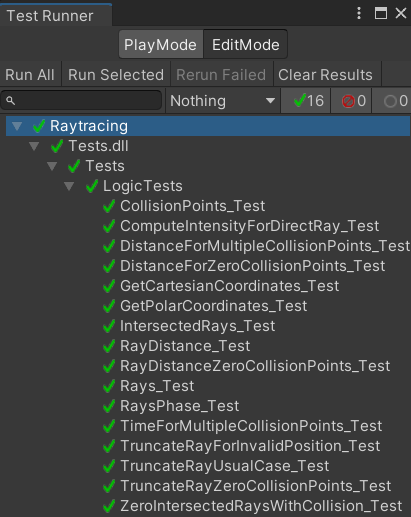
\includegraphics[width=6cm]{imagini/teste1.png}
		\caption{Unit testele aplicației}
		\label{teste}
	\end{figure}
	
	Ca să ne putem asigura de corectitudinea calculelor realizate în cadrul modelului acustic au fost realizate o serie de unit teste menite să verifice anumite situații generale și particulare precum: validarea formulei de calcul a lungimii unei raze, calculul timpilor, ce se întâmpla atunci când avem 0 puncte de coliziune pentru o rază, corectitudinea formulei de calcul a intensității, validarea transformărilor din coordonate polare în carteziene, dar și invers, selecția razelor, intersecția razelor, etc. Toate aceste teste pot fi vizualizate în Figura \ref{teste}.
	
	Rezultatele din aceste camere sunt impresionante, deoarece chiar și pentru camera mică putem face diferența între sunetul de pe primul microfon și cel de pe al doilea microfon. Mai mult, sunetul obținut folosind modelul realizat de noi pentru al treilea microfon este foarte diferit de celelalte microfoane din cameră, ajungând cu un decalaj de timp semnificativ.


\section{Validarea modelului acustic folosind Simcenter 3D}

	Atunci când vorbim despre o aplicație ce propune crearea unui model acustic pentru simularea sunetului în încăperi este foarte important să ne ridicăm problema validării acestuia folosind de exemplu un software similar existent pe piață. În cadrul acestui studiu pentru a fi verificată corectitudinea și validitatea acestui soft am realizat o serie de unit teste ce au fost prezentate în capitolul anterior și, mai mult de atât, am realizat o serie de comparații cu software-ul Simcenter 3D.
	
	Simcenter 3D este o platformă de simulare complet integrată pentru modelarea, simularea și analizarea produselor și sistemelor complexe de inginerie. Platforma include soluții puternice de simulare pentru mai multe discipline, inclusiv analize structurale, acustice, de flux, termice, de mișcare și compoziție, precum și optimizare și simulare multifizică. Software-ul își propune să permită simulărilor să joace un rol timpuriu în procesul de proiectare, ducând la creșterea calității, eficienței și inovației.
	
	Simcenter 3D Acoustics Modeling include toate funcționalitățile necesare pentru a crea, în mod eficient, o geometrie de domeniu fluid prin înfășurarea unei suprafețe cu un mesh structural și/sau un model complet de asamblare CAD.
	
	În cazul simulării acustice Simcenter oferă o bibliotecă extinsă de modele precise pentru estimarea surselor de zgomot aeroacustice, inclusiv modele de stare staționară, modele directe, modele de propagare și rezolvarea ecuațiilor de perturbare acustică. Zgomotul aeroacustic indus de flux este o componentă semnificativă a semnăturii acustice a unui vehicul sau a altor produse. Prezicerea și înțelegerea mecanismelor de generare a zgomotului, localizarea surselor de sunet, identificarea căilor de transmisie și prezicerea răspunsului acustic al sistemului este cheia unui bun design acustic.
	
	Frecvențele care trebuie calculate folosind Simcenter 3D pot fi controlate în totalitate de către utilizator. Acestea pot fi definite manual sau preluate automat din vibrațiile structurale. Într-o interfață grafică de utilizator flexibilă (GUI), utilizatorul poate controla și calcula cantități acustice. Acesta poate analiza rezultatele pentru grupuri de elemente sau microfoane individuale.
	
	Modelul de simulare este verificat automat înainte de exportul în
	solver. Se verifică consistența mesh-ului, materialului și proprietăților. Feedback-ul utilizatorului este furnizat pentru a evita erorile înainte de rezolvare.
	
	Pe lângă funcționalitățile standard de postprocesare pentru vizualizarea
	cantităților acustice precum presiunea, intensitatea și viteza, scenarii specifice pot fi create pentru a filtra și afișa în mod eficient rezultatele funcțiilor legate de microfoane.
	
	Ca să putem realiza o serie de comparații am folosit ambele software-uri și am construit aceeași cameră, poziționând identic sursa audio și microfoanele. Ambele modele acustice au folosit aceeași configurație pentru datele de intrare și au fost urmărite cu mare atenție datele de ieșire. Versiunea de Simcenter ce a fost utilizată pentru această validare a fost Simcenter 3D 2021.1. 
	
	Pentru validarea modelului acustic am creat o cameră rectangulară, folosind ambele soft-uri, cu dimensiunile: 30m lățime, 30m lungime și 15m înălțime, unde am plasat sursa $S$ la poziția $S(0, 2.5,0)$, iar microfoanele au fost așezate astfel: 
	
	\begin{itemize}
		\utb $M0(2, 1.6, 1.7)$, fiind la distanța de 3.07m de sursă
		
		\utb $M1(-1.5, 1.2, 1.7)$, fiind la distanța de 2.56m de sursă
		
		\utb $M2(1, 2, 13)$, fiind la distanța de 13.19m de sursă
	\end{itemize}
	
	În Figura \ref{asemanatoare} putem observa că cele două camere sunt similare, folosesc același sistem de coordonate, sursa și microfoanele sunt poziționate identic.
		
	\begin{figure}[!htb]%
		\begin{subfigure}[b]{.48\textwidth}
			\centering
			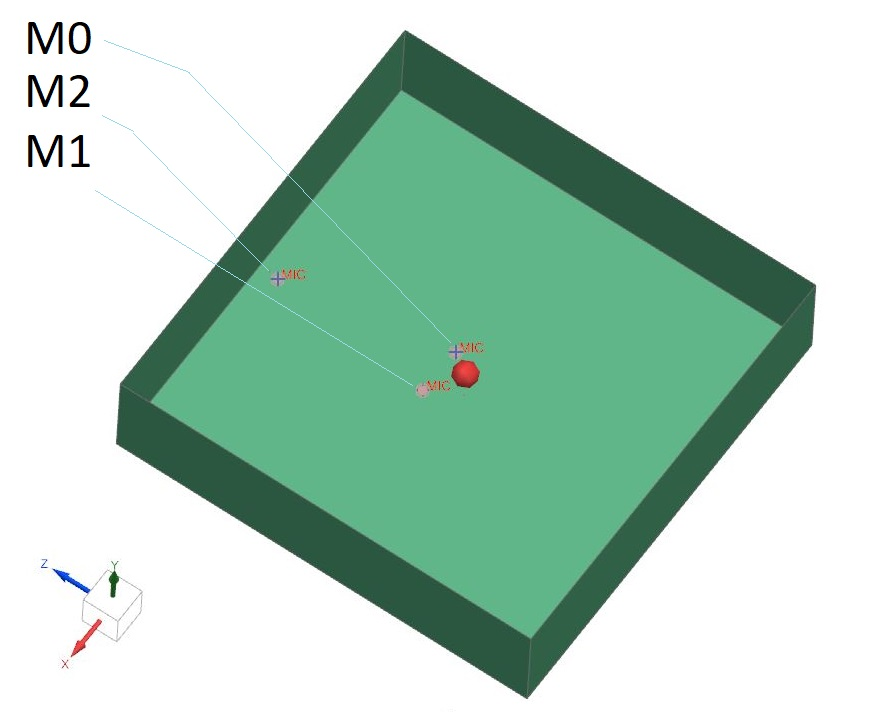
\includegraphics[width=1\linewidth]{imagini/room_view.jpg} 
			%\label{fig:sub-fig}
		\end{subfigure}
		\hfill
		\begin{subfigure}[b]{.48\textwidth}
			\centering
			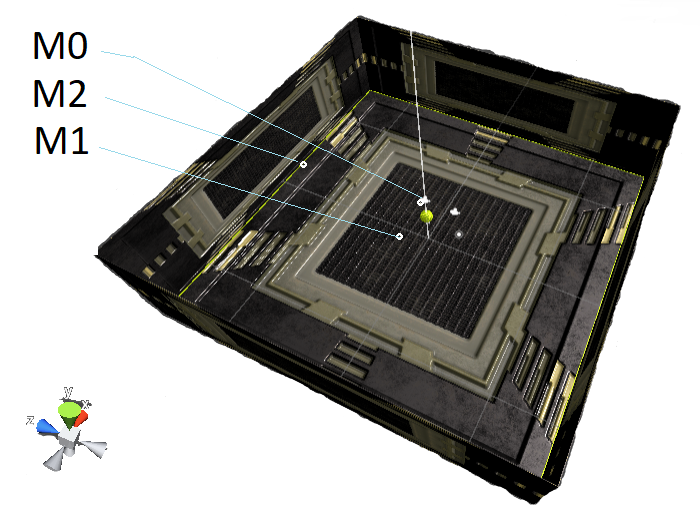
\includegraphics[width=1\linewidth]{imagini/room.png}
			%\label{fig:sub-second}
		\end{subfigure}
		
		\caption{Camerele realizate folosind ambele software-uri}
		\label{asemanatoare}	
	\end{figure}

	
	Vom considera pentru ambele situații c\u{a} densitatea aerului, $\rho_{aer}$, are valoarea $1.2041\dfrac{kg}{m^3}$, iar viteza sunetului prin aer, $c_{aer}$, este $343.21\dfrac{m}{s}$, pentru o temperatur\u{a} constant\u{a} de $20^{\circ}C$.

	Ambele software-uri permit crearea celor două încăperi, crearea unei surse audio și a unor microfoane statice, setarea numărului maxim de reflexii, setarea lungimii maxime a unei raze, setarea pasului de frecvență, folosirea unei melodii, setarea puterii. Diferența dintre cele două software-uri este că Simcenter nu permite setarea numărului de raze ce va fi distribuit în încăpere. Din acest motiv am încercat să găsim un echivalent pentru numărul de raze ce trebuie trasate în încăpere folosind modelul acustic propus de această lucrare. Configurația folosită va fi:
	
	\begin{itemize}
		\utb 1 000 000 de raze distribuite uniform în cazul modelului acustic propus de această lucrare
		
		\utb maxim 10 reflexii pentru o rază
		
		\utb 200m distanța maximă pe care o rază o poate parcurge
		
		\utb 8192Hz numărul de pași de frecvență
	\end{itemize}	

	Configurația folosită pentru camera realizată folosind software-ul Simcenter 3D poate fi viuzalizată cu ajutorul Figurii \ref{config}. Pentru acest software au fost setate dimensiunile potrivite pentru încăpere, numărul maxim de reflexii, distanța maximă, dar și sistemul de coordonate. Putem observa că Simcenter permite utilizarea unor opțiuni mai complexe decât software-ul propus de aplicația descrisă în această lucrare, câteva dintre aceste elemente fiind: opțiunea de a permite difracții 2D și 3D, shimbarea sistemului de coordonate, punerea în evidență a rezultatelor sub mai multe forme, dar și altele.
	
	\begin{figure}[!htb]%
		\begin{subfigure}[b]{.6\textwidth}
			\centering
			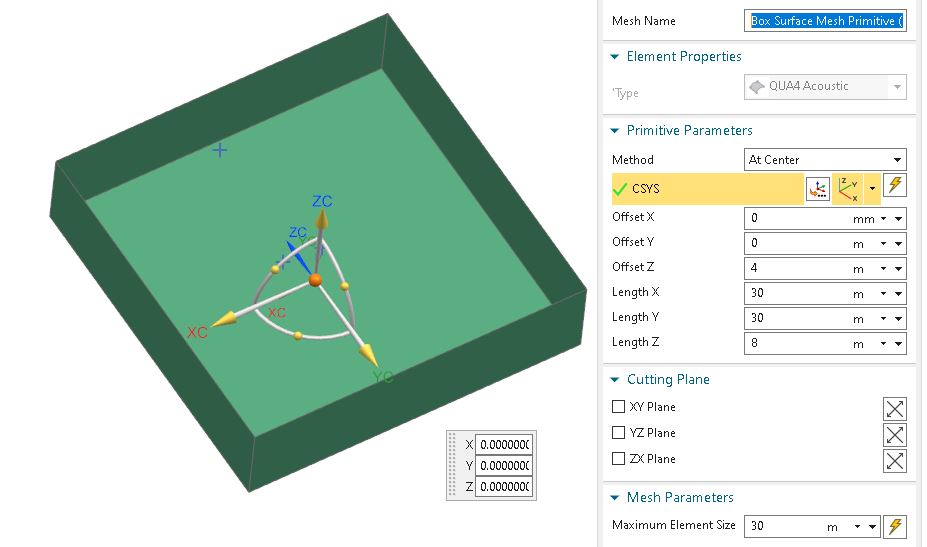
\includegraphics[width=1\linewidth]{imagini/room_primitive.jpg} 
			%\label{fig:sub-fig}
		\end{subfigure}
		\hfill
		\begin{subfigure}[b]{.3\textwidth}
			\centering
			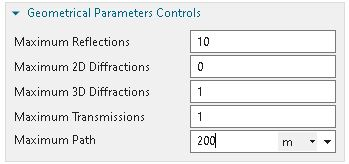
\includegraphics[width=1\linewidth]{imagini/solver_params.jpg}
			%\label{fig:sub-second}
		\end{subfigure}
		
		\caption{Configurația folosită pentru software-ul Simcenter 3D}
		\label{config}	
	\end{figure}
	
	Numărul de raze obținut de modelul vizat de această lucrare pe microfonul $M2$ este 1143, iar numărul de raze care ajunge pe microfonul $M2$ folosind Simcenter este 1400. Conform acestor configurații putem observa similaritatea rezultatelor obținute folosind ambele software-uri urmărind Figura \ref{Fig29}, Figura \ref{Fig26} și Figura \ref{Fig27}.
	
	\begin{figure}[!htb]
		\centering
		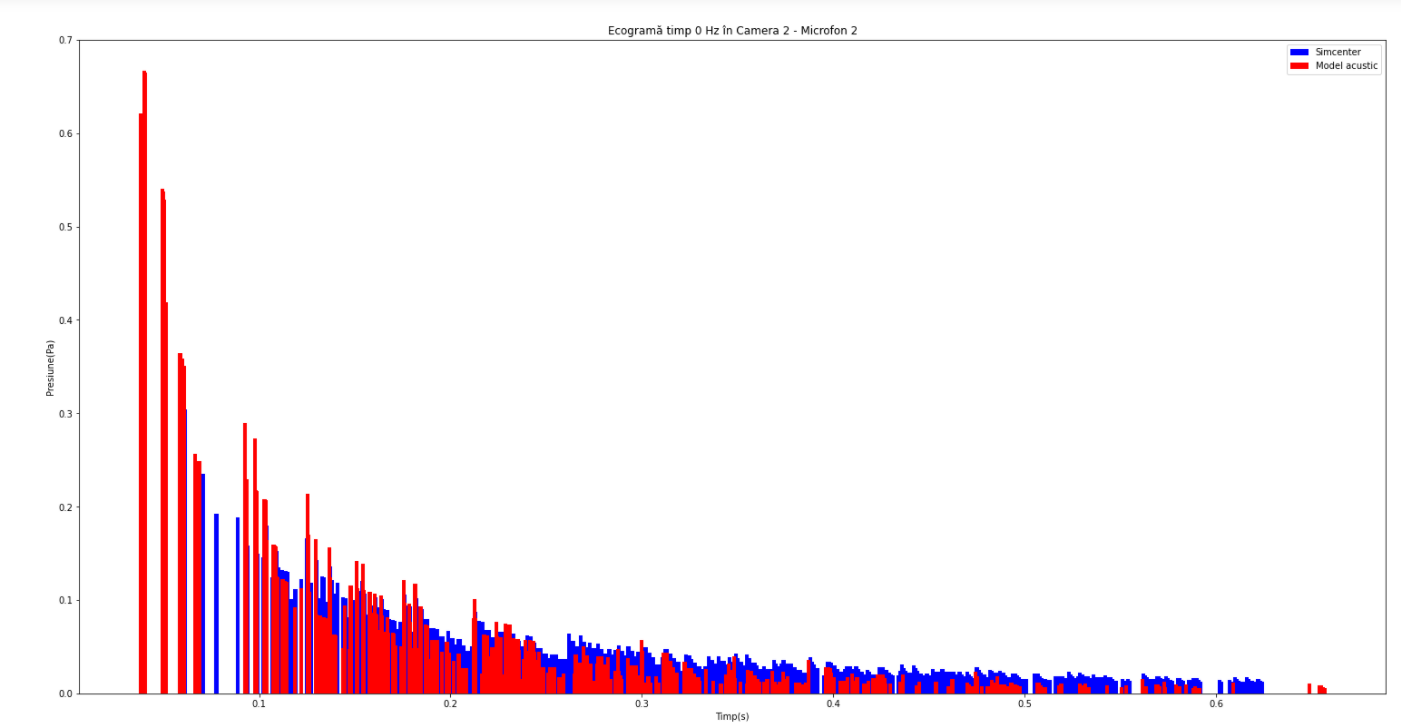
\includegraphics[width=1\linewidth]{imagini/eco_3.png}
		\caption{Ecogramă timp pe microfonul $M2$}
		\label{Fig29}
	\end{figure}

	În cazul ecogramei de timp prezentate în Figura \ref{Fig29}, diferențele de rezultate se explică prin faptul că în Simcenter 3D se folosește un model adaptiv de Ray Tracing care este mai precis. Totuși, pe ecograma se poate observa că nivelul de presiune de la primul impact este același, iar pentru restul impacturilor nivelul este asemănător (diferențele provin din numărul diferit de raze și din traiectoriile diferite). Statistic, pentru un număr suficient de mare de raze din punct de vedere acustic diferențele ar trebui să fie neglijabile.
	
	\begin{figure}[!htb]
		\centering
		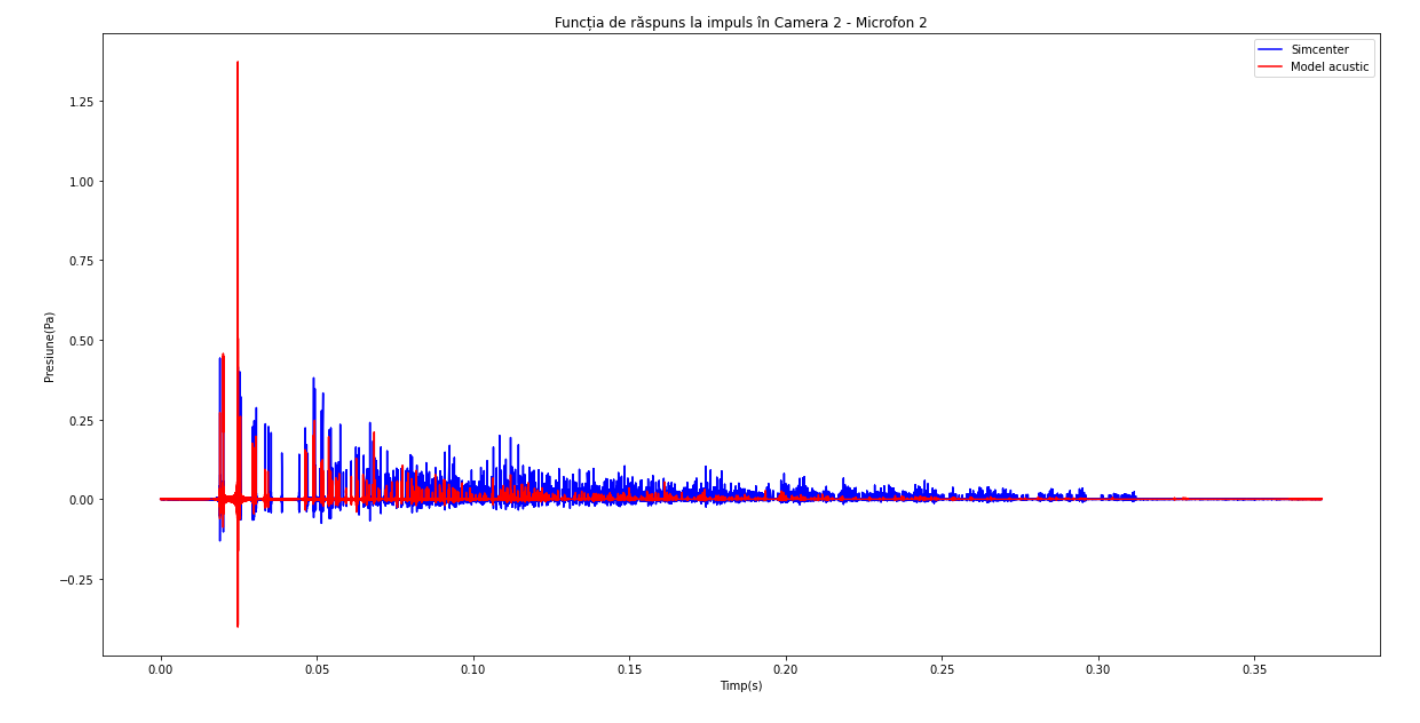
\includegraphics[width=1\linewidth]{imagini/ir_3.png}
		\caption{Funcția de răspuns la impuls pe $M2$}
		\label{Fig26}
	\end{figure}

	Graficul de răspuns la impuls arată amplitudinea undei sonore în timp. Datele utilizate pentru a desena acest grafic sunt produse de un microfon, care probează amplitudinea sunetului la intervale de timp uniform distanțate.

	Precum putem observa în Figura \ref{Fig26}, cele două funcții de răspuns la impuls au valori similare, cu excepția valorii de vârf. Această valoare de vârf diferită este explicată prin faptul că în cazul modelului acustic propus de acest studiu avem 3 raze ce au dimensiuni și căi similare, creând astfel 3 unde care sunt în fază și care își însumează astfel valorile obținând valoarea de vârf din grafic.
	
	Figura \ref{Fig27} prezintă graficul de Frecvență-Magnitudine și graficul Frecvență-Fază cu ajutorul cărora putem reconstrui sunetul audio. Cu ajutorul primul grafic putem să ne dăm seama care este magnitudinea în funcție de frecvență, iar cu ajutorul celui de-al doilea grafic calculăm cât de defazată este o undă sonoră de-a lungul tuturor frecvențelor.
	
	\begin{figure}[!htb]%
		\begin{subfigure}[b]{1\textwidth}
			\centering
			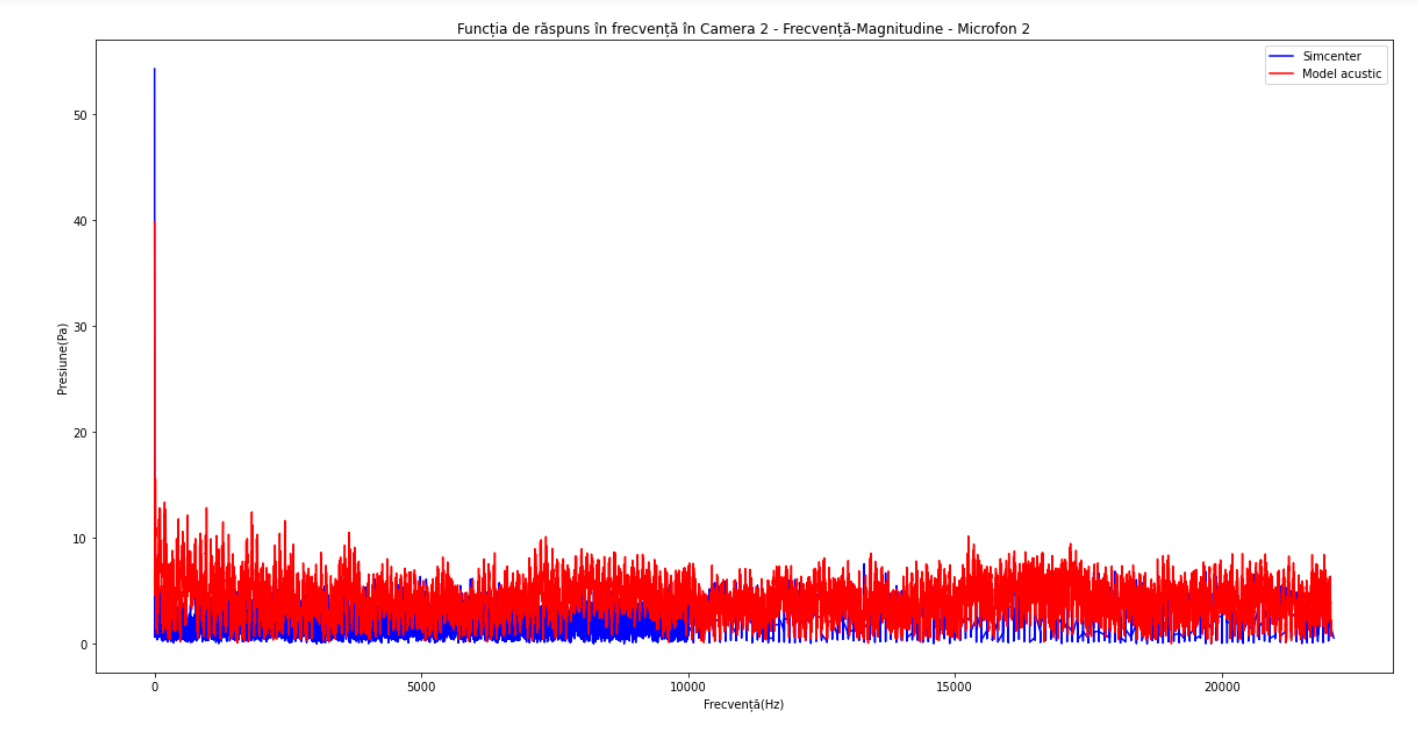
\includegraphics[width=1\linewidth]{imagini/fr_faza_2.png} 
			\caption{Grafic Frecvență-Magnitudine pentru $M2$}
			%\label{fig:sub-fig}
		\end{subfigure}
		\vfill
		\begin{subfigure}[b]{1\textwidth}
			\centering
			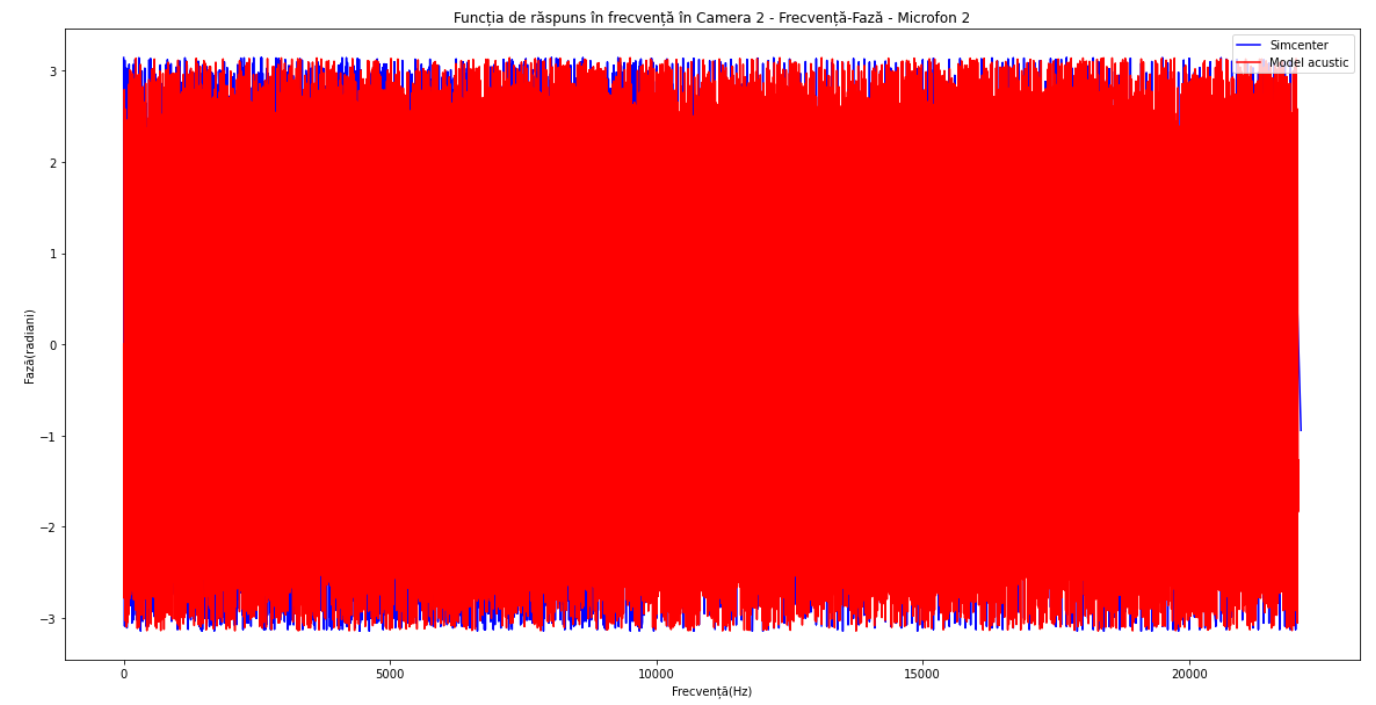
\includegraphics[width=1\linewidth]{imagini/fr_mag_2.png}
			\caption{Grafic Frecvență-Fază pentru $M2$}
			%\label{fig:sub-second}
		\end{subfigure}
		
		\caption{Rezultat Magnitudine-Fază-Frecvență pe $M2$}
		\label{Fig27}	
	\end{figure}

	Considerând toate aceste rezultate prezentate anterior putem să concluzionăm că modelul acustic propus de această lucrare este unul valid, datorită faptului că a trecut cu succes peste toate comparațiile realizate folosind Simcenter 3D. 


